\documentclass{beamer}
\usepackage{etex}

%\useoutertheme[glossy]{wuerzburg}
\useinnertheme[shadow,outline]{chamfered}
%\usecolortheme{shark}
\usecolortheme{beaver}
\beamertemplatenavigationsymbolsempty

\usefonttheme{professionalfonts}
\let\digamma\relax
\usepackage[scale=0.85,stdmathitalics=true,romanfamily=casual]{lucimatx}
\usefonttheme[stillsansseriftext]{serif}

\usepackage{bm}
\usepackage{amsmath}

\usepackage{fancyvrb}

%% Fancy syntax coloring via pygments
%\usepackage{minted}
%\definecolor{bg}{rgb}{0.95,0.95,0.95}
%\usemintedstyle{borland}


% \newenvironment{Rcode}
% {\VerbatimEnvironment
%  \begin{minted}[fontsize=\scriptsize,baselinestretch=1]{r}}%
% {\end{minted}}

% \newenvironment{Pcode}
% {\VerbatimEnvironment
% \begin{minted}[fontsize=\scriptsize,baselinestretch=1]{python}}%
% {\end{minted}}

% \newenvironment{Code}[1]
% {\VerbatimEnvironment
 % \begin{minted}[fontsize=\scriptsize,baselinestretch=1]{#1}}%
% {\end{minted}}


\usepackage{textfit} % commands \scaletoheight{height}{text} and \scaletowidth{width}{text}

\usepackage{tikz}

\usepackage{tcolorbox}

\newtheorem{Alert}{Alert}
\newtheorem{Highlight}{Highlight}

\newcommand{\Species}[1]{{\rmfamily \itshape #1}}
\newcommand{\Real}{\ensuremath{\mathbb{R}}}
\newcommand{\RealN}{\ensuremath{\mathbb{R}^n}}
\newcommand{\RealP}{\ensuremath{\mathbb{R}^p}}
\newcommand{\Mtx}[1]{\ensuremath{\bm{#1}}}
\newcommand{\Inv}[1]{\ensuremath{#1^{-1}}}
\newcommand{\InvMtx}[1]{\ensuremath{\bm{#1}^{-1}}}
\newcommand{\Red}[1]{\textcolor{red}{#1}}
\newcommand{\PsInv}[1]{\ensuremath{\bm{#1}^{+}}}
\DeclareMathOperator{\cov}{cov}
\DeclareMathOperator{\corr}{corr}

\usepackage{booktabs}



% --- Macro \xvec
% From a tex.stackexchange.com answer by Todd Lehman
% http://tex.stackexchange.com/questions/44017/dot-notation-for-derivative-of-a-vector
\makeatletter
\newlength\xvec@height%
\newlength\xvec@depth%
\newlength\xvec@width%
\newcommand{\xvec}[2][]{%
  \ifmmode%
    \settoheight{\xvec@height}{$#2$}%
    \settodepth{\xvec@depth}{$#2$}%
    \settowidth{\xvec@width}{$#2$}%
  \else%
    \settoheight{\xvec@height}{#2}%
    \settodepth{\xvec@depth}{#2}%
    \settowidth{\xvec@width}{#2}%
  \fi%
  \def\xvec@arg{#1}%
  \def\xvec@dd{:}%
  \def\xvec@d{.}%
  \raisebox{.2ex}{\raisebox{\xvec@height}{\rlap{%
    \kern.05em%  (Because left edge of drawing is at .05em)
    \begin{tikzpicture}[scale=1]
    \pgfsetroundcap
    \draw (.05em,0)--(\xvec@width-.05em,0);
    \draw (\xvec@width-.05em,0)--(\xvec@width-.15em, .075em);
    \draw (\xvec@width-.05em,0)--(\xvec@width-.15em,-.075em);
    \ifx\xvec@arg\xvec@d%
      \fill(\xvec@width*.45,.5ex) circle (.5pt);%
    \else\ifx\xvec@arg\xvec@dd%
      \fill(\xvec@width*.30,.5ex) circle (.5pt);%
      \fill(\xvec@width*.65,.5ex) circle (.5pt);%
    \fi\fi%
    \end{tikzpicture}%
  }}}%
  #2%
}
\makeatother

% --- Override \vec with an invocation of \xvec.
\let\stdvec\vec
\renewcommand{\vec}[1]{\xvec[]{\bm{#1}}}
% --- Define \dvec and \ddvec for dotted and double-dotted vectors.
\newcommand{\dvec}[1]{\xvec[.]{#1}}
\newcommand{\ddvec}[1]{\xvec[:]{#1}}


\usepackage{pifont}
\newcommand{\weblink}{\ding{43}}  % hand with pointing finger

\definecolor{links}{HTML}{2A1B81}
\hypersetup{colorlinks,linkcolor=,urlcolor=magenta}

\usepackage{tikz}

\usepackage{amsfonts}
\usepackage{tikz}
\usepackage{caption}
\usepackage{subcaption}

\usepackage[inline]{asymptote}
\usepackage{attachfile2}
\usepackage{asyfig}





%===========================================================
% Title Info
\title{Scientific Computing for Biologists}
\subtitle{Multiple Regression} % (optional)

\author{Paul M. Magwene}


\date{}

\begin{document}
%===========================================================
\begin{frame}
\titlepage
\end{frame}



%===========================================================
\begin{frame}[fragile]
  \frametitle{Variable space view of multiple regression}

\begin{center}
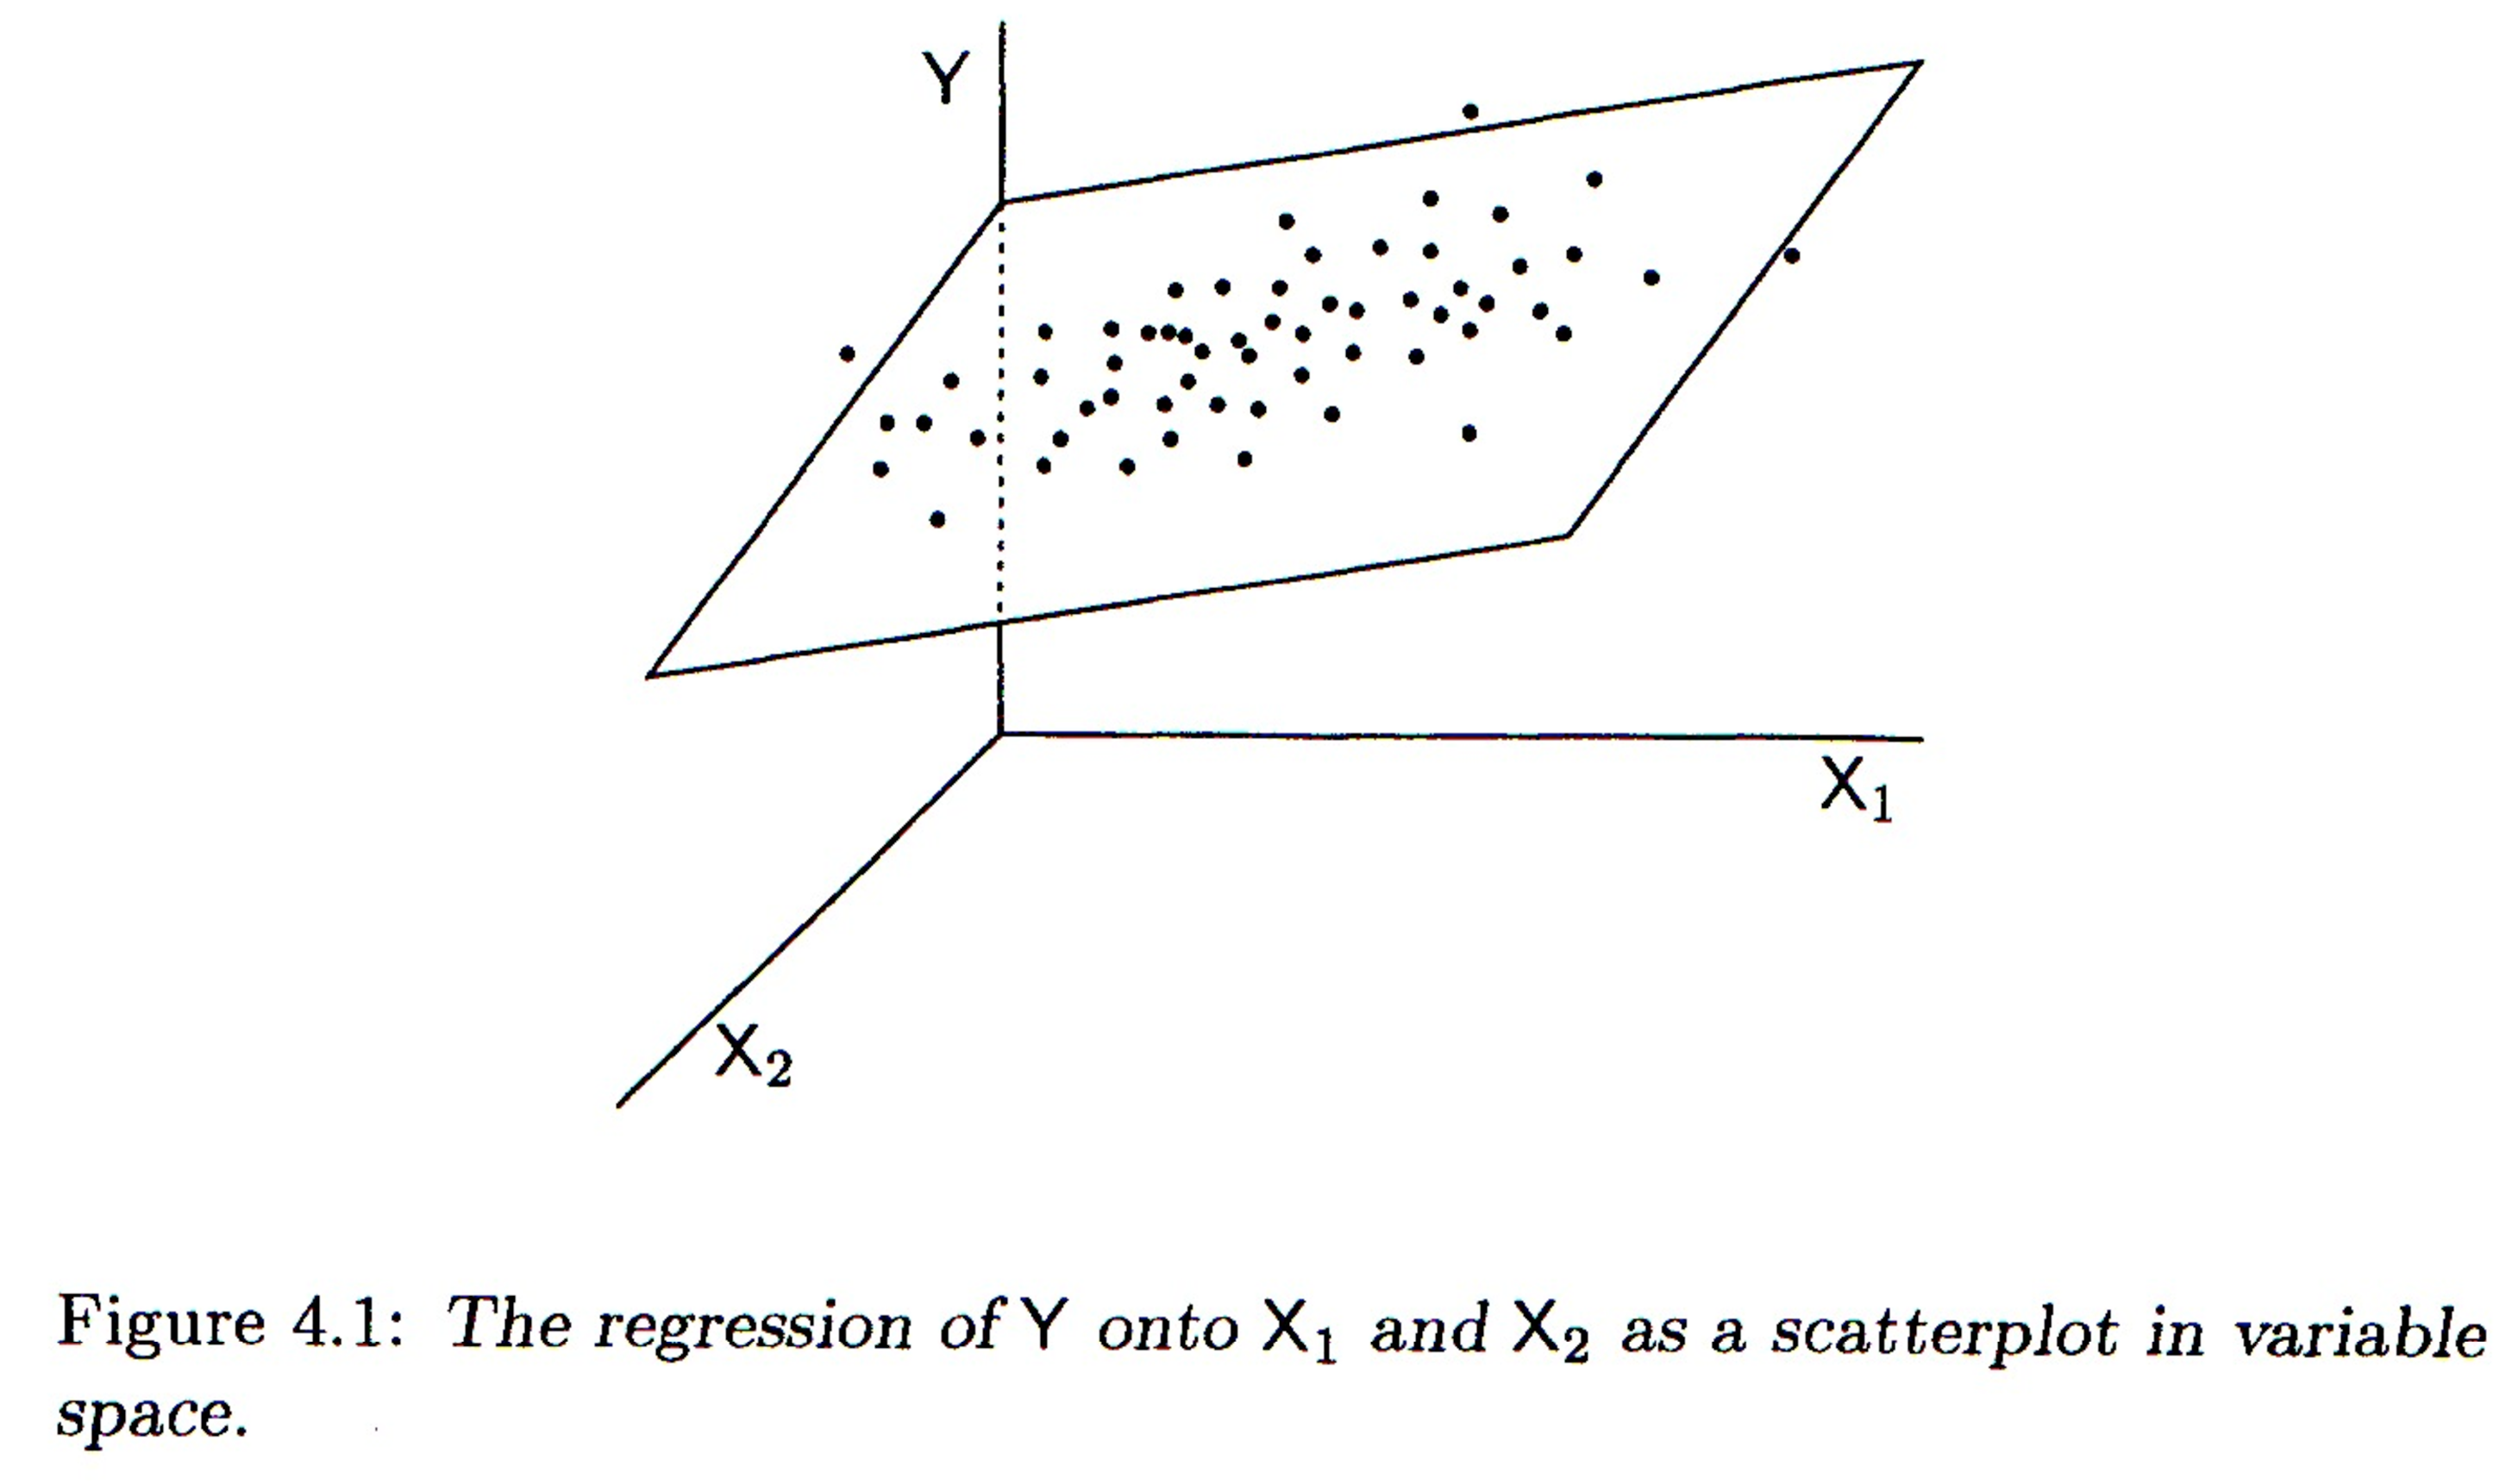
\includegraphics[height=2.5in]{regression-variable-space.pdf}
\end{center}


\end{frame}
%===========================================================


%===========================================================
\begin{frame}
  \frametitle{Subject Space Geometry of Multiple Regression}

\begin{center}
\asyinclude[height=2.5in,inline=true]{multiregr.asy}
\end{center}

\[
\vec{y} = \hat{\vec{y}} + \vec{e}
\]

\end{frame}

%===========================================================
\begin{frame}
  \frametitle{Multiple Regression}


$$
\hat{\vec{y}} = a\Mtx{1} + b_1\Mtx{X}_1 + b_2\Mtx{X}_2 + \cdots + b_p\Mtx{X}_p
$$

\medskip

\[
\left[ 
\begin{array}{c}
\hat{y}_1 \\ \hat{y}_2 \\ \vdots \\\hat{y}_n \\
\end{array}
\right]
=
a\left[
\begin{array}{c}
1 \\ 1 \\ \vdots \\1 \\
\end{array}
\right]
+
b_1\left[
\begin{array}{c}
x_{11}\\ x_{21} \\ \vdots \\x_{n1} \\
\end{array}
\right]
+
b_2\left[
\begin{array}{c}
x_{12}\\ x_{22} \\ \vdots \\x_{n2} \\
\end{array}
\right]
+
\cdots
+
b_p\left[
\begin{array}{c}
x_{1p}\\ x_{2p} \\ \vdots \\x_{np} \\
\end{array}
\right]
\]

\end{frame}
%===========================================================

%===========================================================
\begin{frame}[fragile]
    \frametitle{$\hat{y}$ is linear combination of the predictor variables}

Recall that a \emph{linear combination} of vectors is an equation of the form:

\[
z = b_1 \Mtx{x}_1 + b_2 \Mtx{x}_2 + \cdots + b_p \Mtx{x}_p
\]

\medskip

In regression, the vector of fitted values, $\hat{\vec{y}}$, is a linear combination of the predictor variables.

\end{frame}
%===========================================================

%===========================================================
\begin{frame}
  \frametitle{Matrix Representation of Multiple Regression}

Let $\vec{y}$ be a vector of values for the outcome variable. Let $\Mtx{X}_i$ be explanatory variables. In matrix form:

$$
\vec{y}  = \Mtx{X}\vec{b} + \vec{e}
$$

$$
\vec{y} = \left[ \begin{array}{c}
y_1 \\ y_2 \\ \vdots \\y_n \\
\end{array}
\right]
\;
;
\;
\Mtx{X} = \left[ \begin{array}{ccccc}
1 & x_{11} & x_{12} & \cdots & x_{1p} \\
1 & x_{21} & x_{22} & \cdots & x_{2p} \\
\vdots & \vdots & \vdots & \vdots & \vdots \\
1 & x_{n1} & x_{n2} & \cdots & x_{np} \\
\end{array}
\right]
\;
;
$$

$$
\Mtx{b} = \left[ \begin{array}{c}
a \\ b_1 \\ b_2 \\ \vdots \\ b_p \\
\end{array}
\right]
\;
;
\;
\Mtx{e} = \left[ \begin{array}{c}
e_1 \\ e_2 \\ \vdots \\e_n \\
\end{array}
\right]
$$

\end{frame}
%===========================================================
\begin{frame}
  \frametitle{Estimating the Coefficients for Multiple Regression}


$$
\vec{y} = \Mtx{X}\vec{b} + \vec{e}
$$
\bigskip

Estimate $\vec{b}$ as:
$$
\vec{b} = (\Mtx{X}^T \Mtx{X})^{-1}\Mtx{X}^T\vec{y}
$$

\end{frame}
%===========================================================


%===========================================================
\begin{frame}
  \frametitle{Matrix Inverses}

\begin{itemize}
\item If $A$ is a \emph{square matrix} and $C$ is a matrix of the same size where $AC = I$ and $CA=I$ than $C$ is the inverse of $A$ and we denote is \Inv{A}.

\[
A\Inv{A} = \Inv{A}A = I
\]


\item Rules for inverses:

\begin{itemize}
 \item Only square matrices are invertible
 \item A matrix for which we can find an inverse is called \emph{\textbf{invertible}} (non-singular)
 \item A matrix for which no inverse exists is \emph{\textbf{singular}} (non-invertible)
 \item If $A$ and $B$ are both invertible $p \times p$ matrices than $\Inv{(AB)} = \Inv{B} \Inv{A}$ (note change in order).
\end{itemize}
 
\end{itemize}


\end{frame}
%===========================================================

%===========================================================
\begin{frame}
  \frametitle{More facts about Matrix Inverses}

 \begin{itemize}
 \item Not every square matrix is invertible
 \item Every orthogonal matrix is invertible
 \item Any diagonal matrix, $A$, where the $a_{ii}$ are non-zero, is invertible
 \end{itemize}
 
\end{frame} 

%===========================================================

%===========================================================
\begin{frame}
  \frametitle{Regression coefficients}

\[
\vec{b} = \left[ \begin{array}{c}
a \\ b_1 \\ b_2 \\ \vdots \\ b_p \\
\end{array}
\right] 
\]


\begin{itemize}
    \item The regression coefficients can be thought of as ``weightings'' of the predictor variables
    \item Comparing the magnitude of regression coefficients only makes sense if all the predictor variables have the same scale
    \item If predictor variables have different scales, then can can first standardize the variables (subtract means and divide by variances), before fitting regression to get standardized regression coefficients.  
    \item Alternately, calculate standardized regression coefficients as:
        \[
        b'_j = \frac{|\vec{x}_j|}{|\vec{y}|} b_j
        \]
\end{itemize}

\end{frame}
%===========================================================



%===========================================================
\begin{frame}
  \frametitle{Regression loadings}

The correlation between each predictor variable, $\Mtx{x}_j$and the prediction, $\hat{\vec{y}}$, is given by the angle between them:

        \[
        \cos \theta_{\vec{x_j},\vec{\widehat{y}}} = \frac{\vec{x_j} \cdot \vec{\widehat{y}}}{|\vec{x_j}||\vec{\widehat{y}}|}
        \]

\medskip

These are sometimes called ``loadings'' and should be examined in combination with the regression coefficients to understand the model implied by the multiple regression.

\begin{center}
\asyinclude[viewportwidth=0.3\textwidth,height=1.25in,keepAspect=true,inline=true]{multiregr-loadings.asy}
\end{center}


\end{frame}
%===========================================================

%===========================================================
\begin{frame}
  \frametitle{Space Spanned by a List of Vectors}


\begin{block}{Definition}
Let $X$ be a finite list of $n$-vectors. The \textbf{space spanned} by $X$ is the set of all vectors that can be written as linear combinations of the vectors in $X$.
\end{block}

\smallskip

\begin{center}
\asyinclude[height=1.25in,inline=true]{multiregr.asy}
\end{center}

\smallskip

The prediction, $\hat{\vec{y}}$ is the closest vector to $\vec{y}$ in the space spanned by the predictor variables, $\Mtx{X}$.

\end{frame}

%===========================================================





%===========================================================
\begin{frame}
  \frametitle{The predictor variables must be linearly independent}

To solve the multiple regression equation, the predictor variables, $\Mtx{X}$, must be linearly independent.

\begin{itemize}

\item A list of vectors, $\Mtx{x}_1, \Mtx{x}_2, ..., \Mtx{x}_p$ , is said the be \emph{\textbf{linearly dependent}} if there is a non-trivial combination of them which is equal to the zero vector.
\[
 b_1 \Mtx{x}_1 + b_2 \Mtx{x}_2 + \cdots + b_p \Mtx{x}_p = 0
\]

\item When a set of vectors are linearly dependent we also called them  \emph{\textbf{multicollinear}}

\item A list of vectors that are \emph{not} linearly dependent are said to be \emph{\textbf{linearly independent}}

\item  If a matrix is invertible than it's columns form a linearly independent list of vectors!

\end{itemize}


\end{frame}
%===========================================================



%===========================================================

\begin{frame}
  \frametitle{Near multicollinearity of the predictors leads to unstable regression solutions}

Predictor variables that are \textbf{nearly multicollinear} are, perhaps, even more difficult to deal with:  

\begin{figure}
\begin{center}
\subcaptionbox{Non-collinear predictors}{\asyinclude[height=1.35in,keepAspect=true]{regr-noncolinear.asy}}
\subcaptionbox{Nearly collinear predictors}{\asyinclude[height=1.35in,keepAspect=true]{regr-colinear.asy}}
\end{center}
\caption{When predictors are nearly collinear, small differences in the vectors can result in large differences in the estimated regression.}
\end{figure}

\end{frame}
%===========================================================




%===========================================================
\begin{frame}
  \frametitle{What can I do if my predictors are (nearly) collinear?}

\begin{itemize}
    \item Drop some of the linearly dependent sets of predictors.
    \item Replace the linearly dependent predictors with a combined variable.
    \item Define orthogonal predictors, via linear combinations of the original variables (PC regression approach)
    \item `Tweak' the predictor variables so that they're no longer multicollinear (Ridge regression).
\end{itemize}

\end{frame}
%===========================================================






%===========================================================
\begin{frame}
  \frametitle{Curvilinear Regression}

Curvilinear regression using \textbf{polynomial models} is simply multiple regression with the $x_i$ replace by powers of $x$.
\bigskip

$$
\hat{y} = b_1\Mtx{x} + b_2\Mtx{x}^2 + \cdots + b_p\Mtx{x}^n
$$

\medskip

Note:
\begin{itemize}
	\item this is still a \emph{linear} regression (linear in the coefficients)
	\item best applied when a specific hypothesis justifies their use
	\item generally not higher than quadratic or cubic
\end{itemize}

\end{frame}
%===========================================================
\begin{frame}[fragile]
  \frametitle{Example of Curvilinear Regression}

\begin{center}
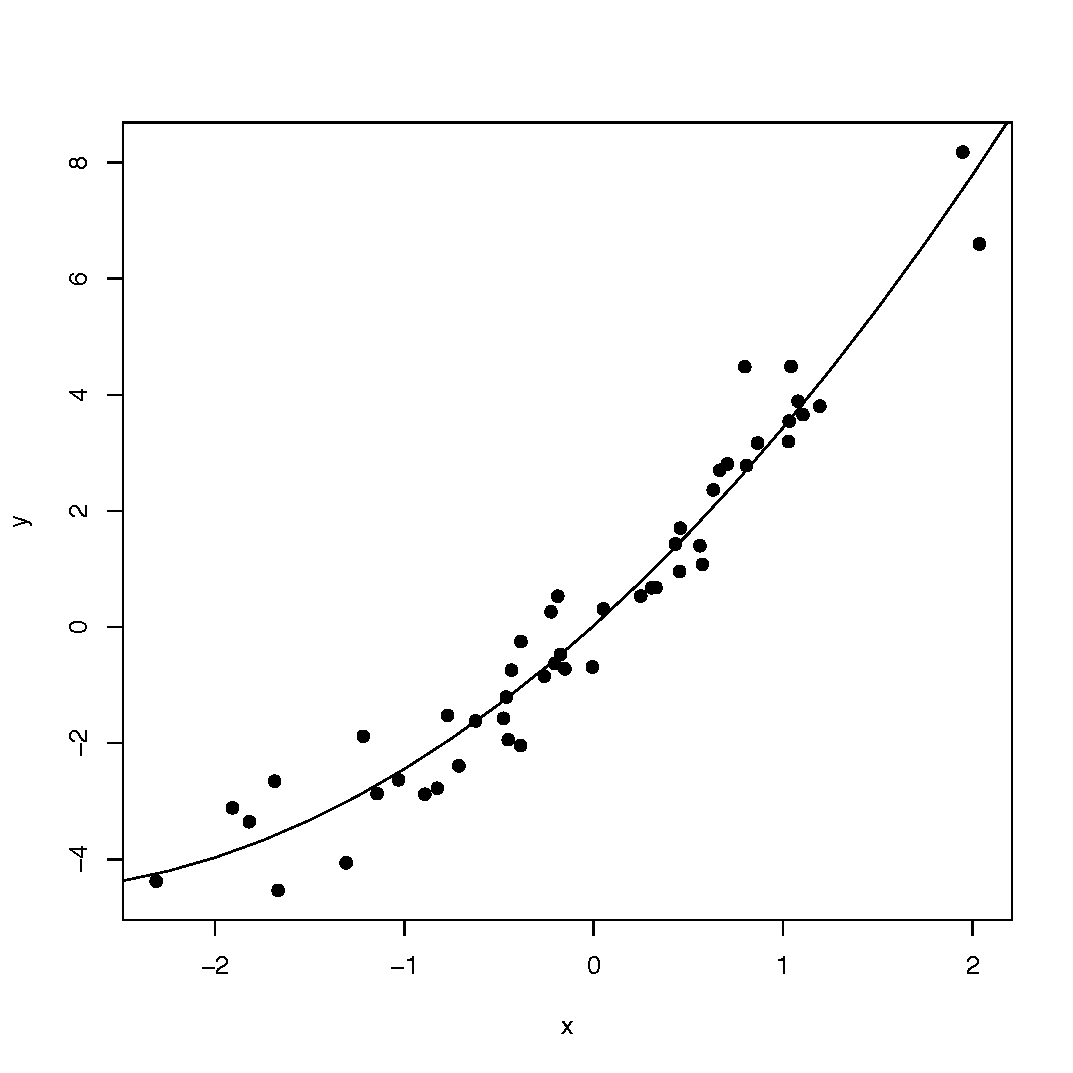
\includegraphics[height=1.75in]{curvilinear-regression.pdf}\\
 $\Mtx{y} = 3\Mtx{x} + 0.5\Mtx{x}^2 + \Mtx{e}$
\end{center}

\begin{verbatim}
lm(formula = y ~ x + I(x^2))
Coefficients:
            Estimate Std. Error t value Pr(>|t|)
(Intercept)  0.02229    0.11651   0.191    0.849
x            2.94001    0.09693  30.331  < 2e-16 ***
I(x^2)       0.47146    0.07685   6.135 1.68e-07 ***
\end{verbatim}


\end{frame}
%===========================================================



\end{document}


%===========================================================
\begin{frame}
  \frametitle{XXX}

\end{frame}
%===========================================================
